\apendicemanual{Manual visual do Memora atualizado}{ap:manual-visual}
As quatro capturas anotadas ilustram a configuração, a execução, a análise e a conclusão de um cenário de 21 acessos. Foram produzidas em navegador com resolução de 1600$\times$900 e representam a evolução da interface, sem documentar as telas de cada entrevista.

\subsection*{Configurar, passos 1--5}
\begin{figure}[!htbp]
\centering
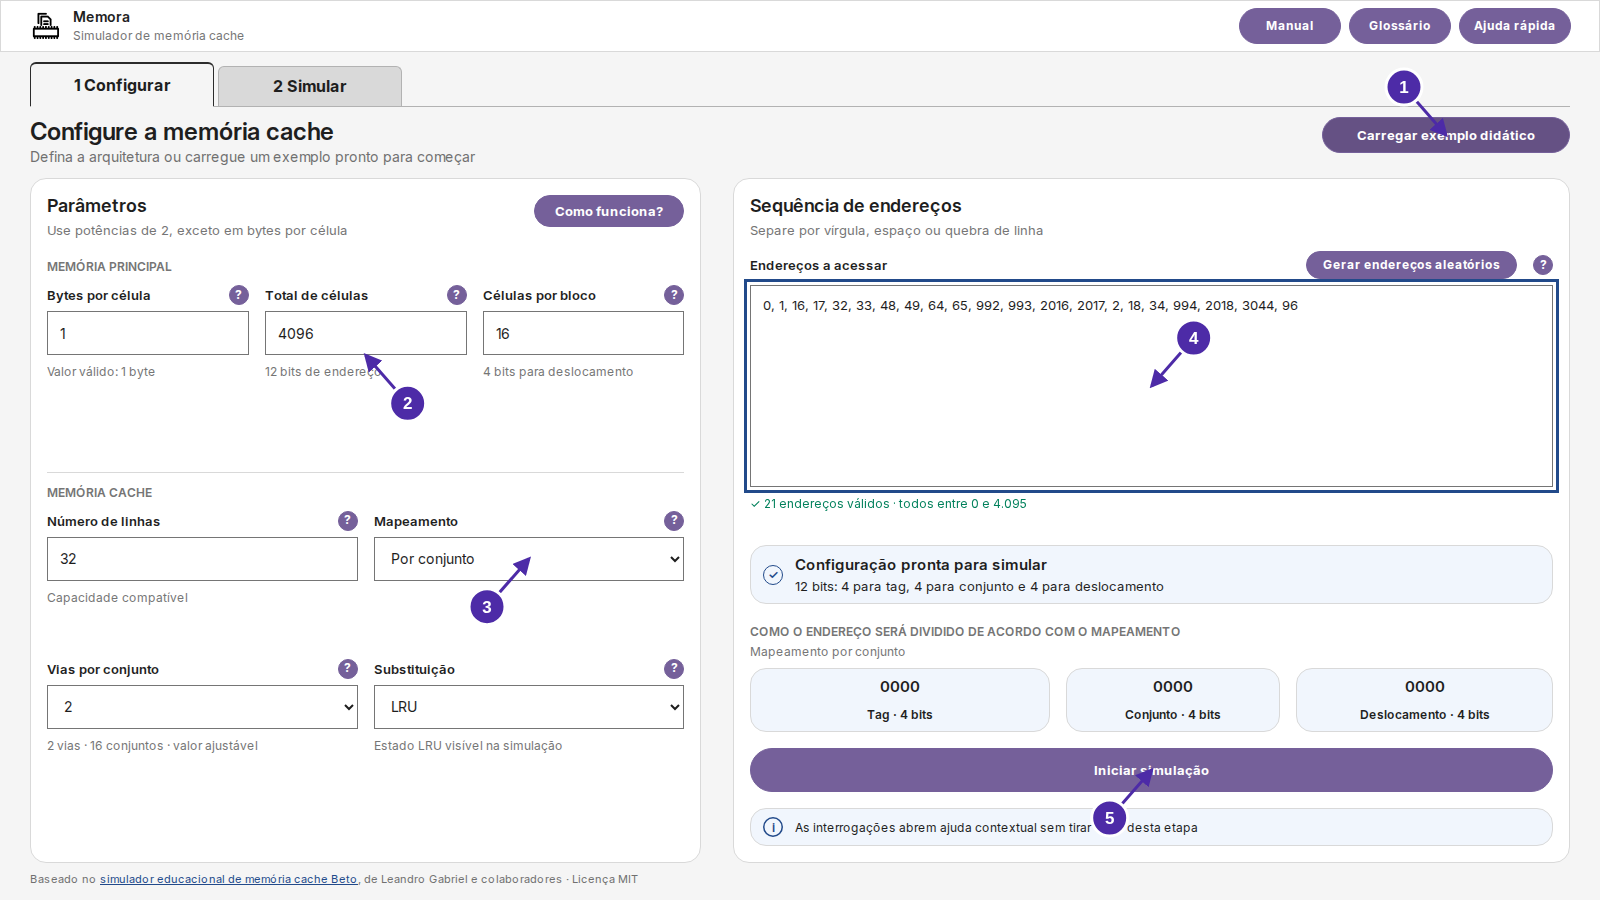
\includegraphics[width=\linewidth,height=0.39\textheight,keepaspectratio]{figuras/manual/configurar.png}
\caption{Manual de Configurar: passos 1--5.}
\label{fig:manual-configurar}
\par\footnotesize Fonte: captura própria da aplicação; cenário ilustrativo.
\end{figure}
\begin{enumerate}
\item Carregar exemplo didático.
\item Conferir memória, cache e ajuda dos campos.
\item Escolher mapeamento por conjunto, duas vias e LRU.
\item Editar endereços e conferir a prévia da divisão.
\item Iniciar simulação.
\end{enumerate}

\clearpage
\subsection*{Simular, passos 1--6}
\begin{figure}[!htbp]
\centering
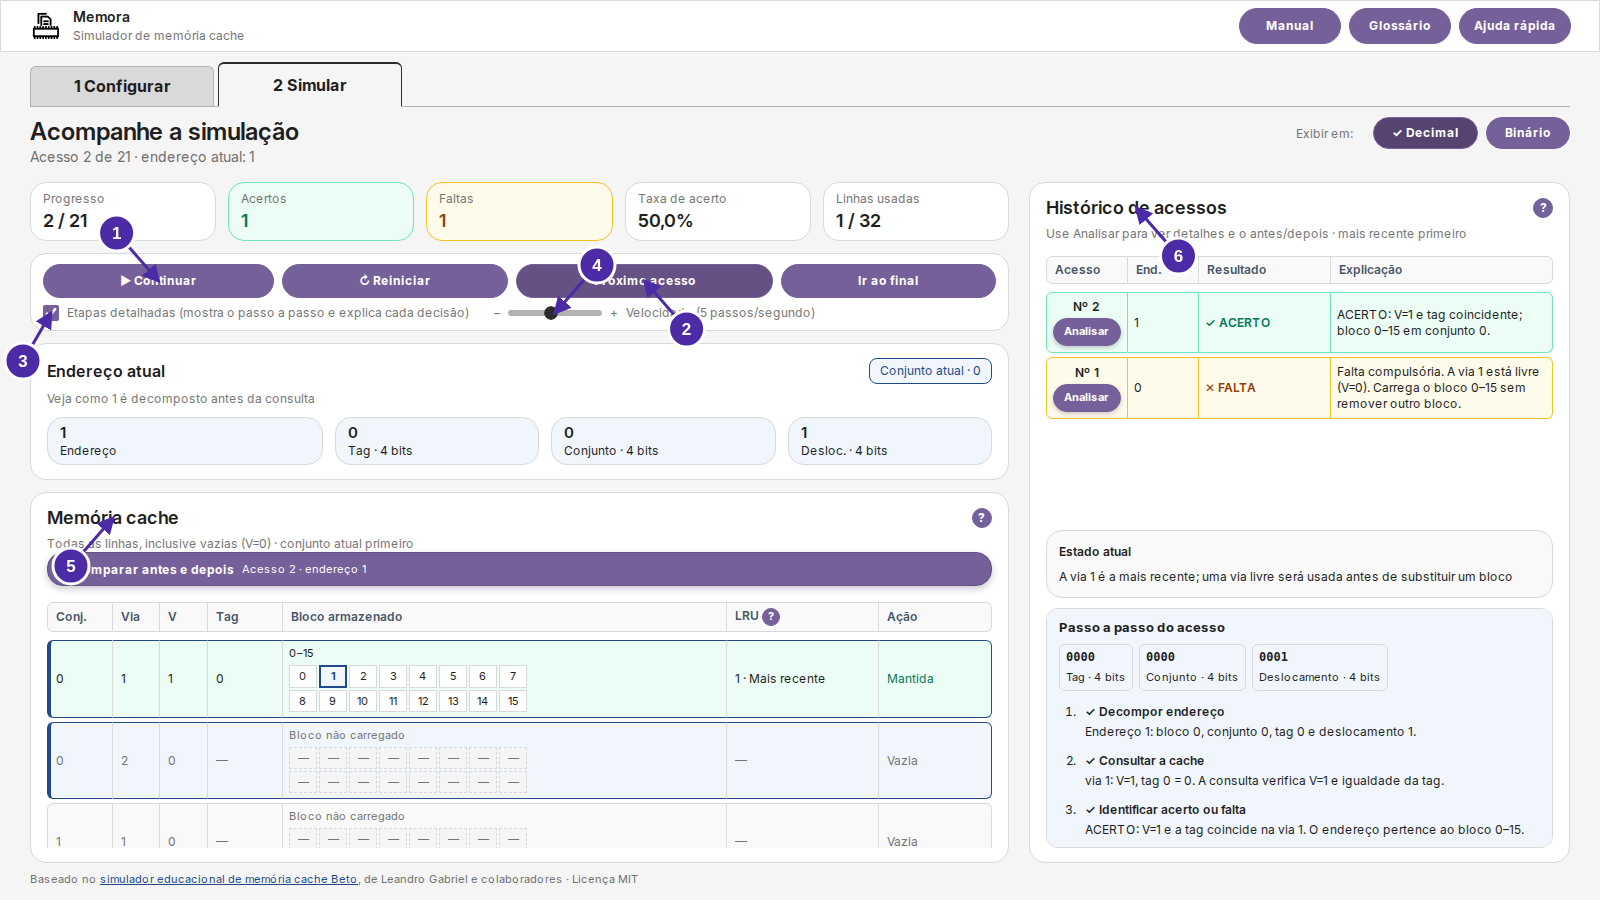
\includegraphics[width=\linewidth,height=0.39\textheight,keepaspectratio]{figuras/manual/simular.png}
\caption{Manual de Simular: passos 1--6.}
\label{fig:manual-simular}
\par\footnotesize Fonte: captura própria da aplicação; cenário ilustrativo.
\end{figure}
\begin{enumerate}
\item Iniciar, pausar e continuar.
\item Avançar, ir ao final ou reiniciar.
\item Ativar etapas detalhadas.
\item Regular a velocidade.
\item Examinar o estado da cache e LRU.
\item Selecionar Analisar abaixo de Nº N no histórico.
\end{enumerate}

\clearpage
\subsection*{Analisar, passos 7--9}
\begin{figure}[!htbp]
\centering
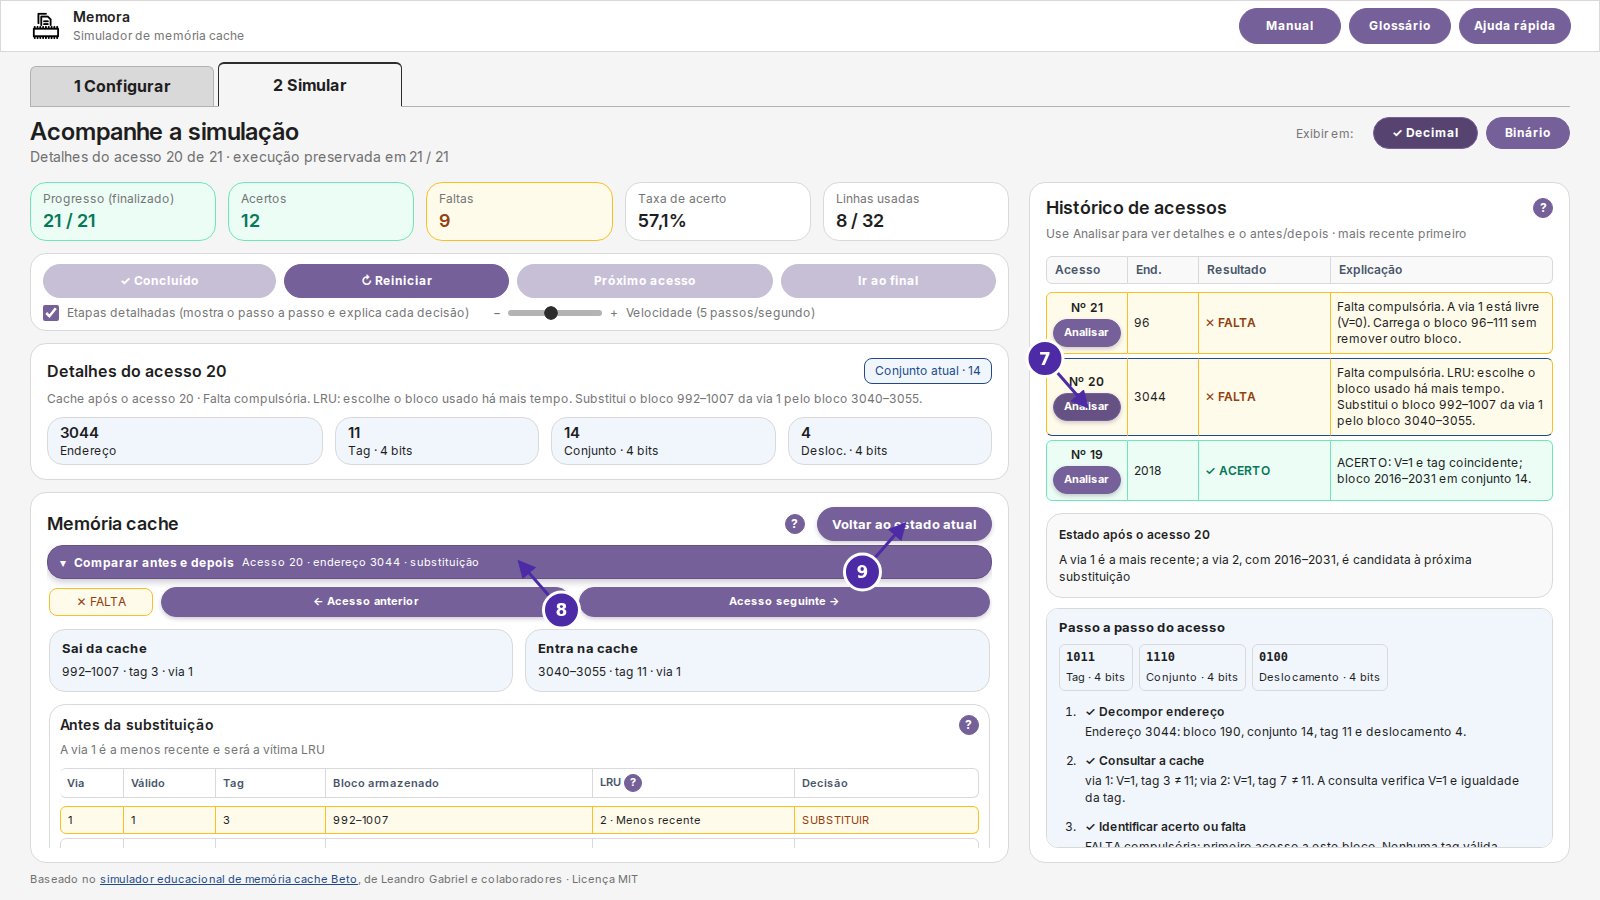
\includegraphics[width=\linewidth,height=0.39\textheight,keepaspectratio]{figuras/manual/comparacao.png}
\caption{Manual: comparação do acesso 20, passos 7--9.}
\label{fig:manual-comparacao}
\par\footnotesize Fonte: captura própria da aplicação; cenário ilustrativo.
\end{figure}
\begin{enumerate}
\item Selecionar Analisar no acesso 20.
\item Comparar a saída do bloco 992--1007 com a entrada do bloco 3040--3055.
\item No cabeçalho de Memória cache, escolher Voltar ao estado atual. A ação fecha a comparação e preserva os contadores.
\end{enumerate}

\clearpage
\subsection*{Conclusão, passo 10}
\begin{figure}[!htbp]
\centering
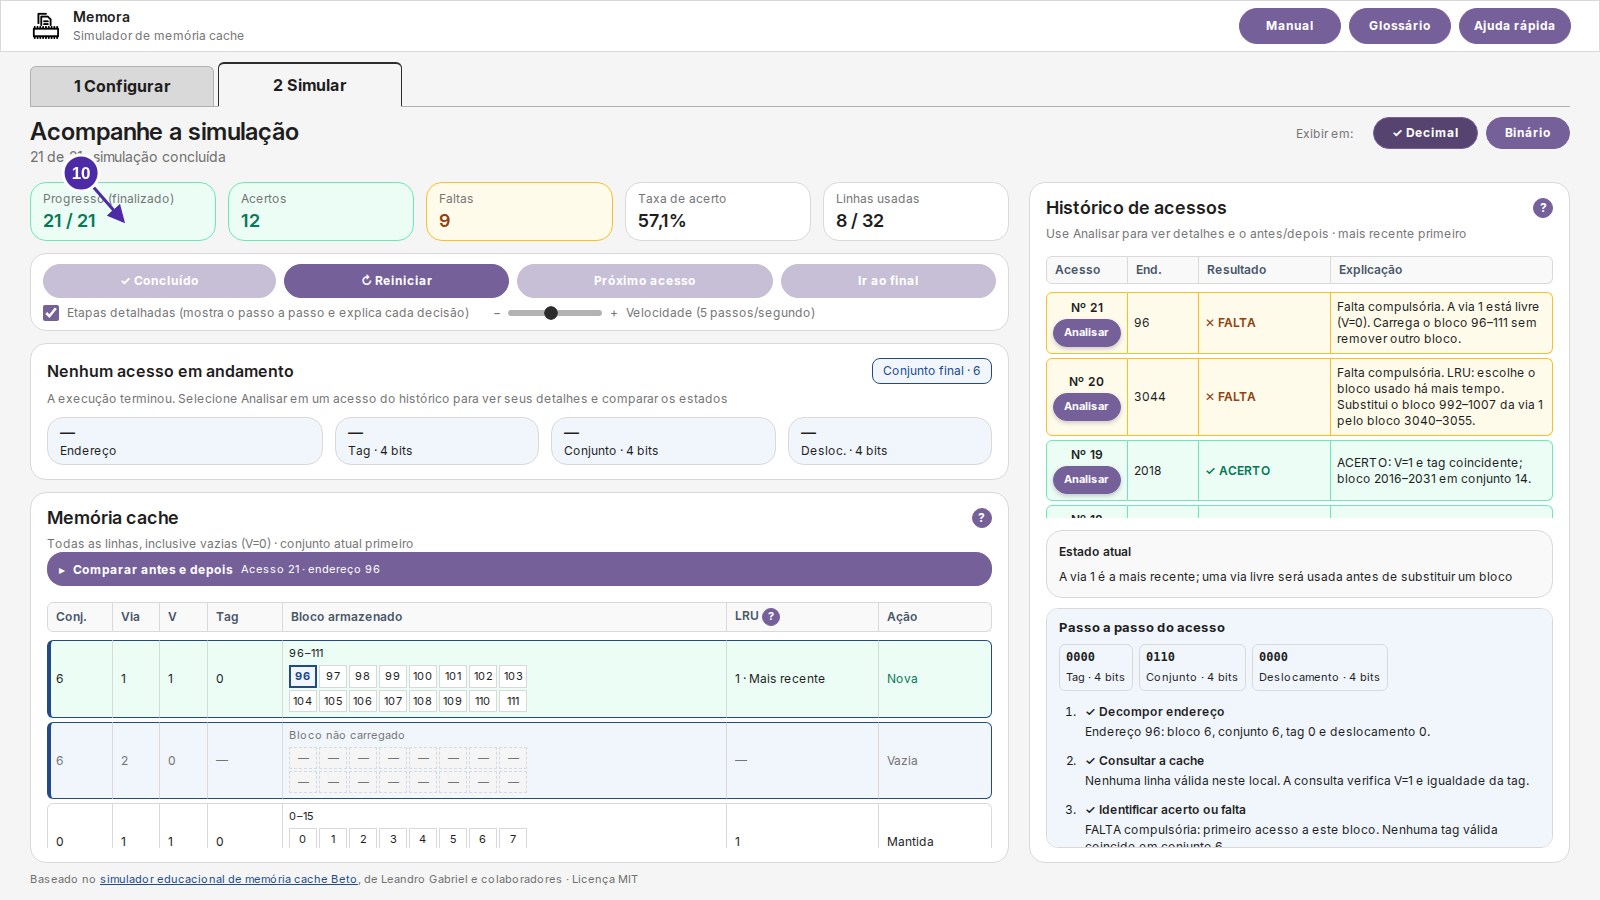
\includegraphics[width=\linewidth,height=0.39\textheight,keepaspectratio]{figuras/manual/conclusao.png}
\caption{Manual: conclusão 21/21, passo 10.}
\label{fig:manual-conclusao}
\par\footnotesize Fonte: captura própria da aplicação; cenário ilustrativo.
\end{figure}
O histórico e os totais permanecem disponíveis após o progresso chegar a 21/21.


